\documentclass[11pt,a4paper]{article}
\usepackage[T1]{fontenc}
\usepackage[utf8]{inputenc}
\usepackage{lmodern,microtype}
\usepackage{amsmath,amssymb,mathtools,amsthm}
\usepackage{geometry,booktabs,tabularx,array,graphicx,hyperref}
\geometry{margin=2.4cm}
\hypersetup{colorlinks=true,linkcolor=black,citecolor=black,urlcolor=blue}
\newtheorem{theorem}{Theorem}[section]
\newtheorem{corollary}[theorem]{Corollary}
\title{\textbf{Geometry of Continuous 3-SAT Relaxations}\\[0.3em]\large Hinge Plateaus, Harmonic Multilinear Landscapes, and Softplus Convexity}
\author{Thiago Carvalho\\Independent Researcher\\\texttt{thiagocarvalho.dba@gmail.com}}
\date{Draft for analysis -- derived from audited CLG-R v4.0.5 source (September 2026)}
\begin{document}\maketitle
\begin{abstract}
We compare three continuous representations of 3-SAT on the hypercube $[-1,1]^N$: a squared Hinge penalty of the clause-wise linear relaxation, the natural multilinear extension of the Boolean violation count, and a Softplus smoothing of the same affine clause violations. Although all three are tied to the same discrete clause structure, their interior geometries are qualitatively different. We prove that the Hinge relaxation contains the universal central fractional box $(-1/3,1/3)^N$ on which both energy and gradient vanish, providing a direct geometric manifestation of the $0.5$ interior slack of the clause-wise LP relaxation. Under a non-degeneracy condition on the Boolean objective, the critical sets of the multilinear and Softplus relaxations have Lebesgue measure zero. The multilinear extension is harmonic, hence has no interior local minima; every non-degenerate interior critical point is a saddle, and every strict local minimum on the projected cube is a Boolean vertex. By contrast, the Softplus Hessian factors globally as $V^TW(x)V\succeq0$ and becomes positive definite when the clause incidence matrix has full column rank. We derive explicit spectral and Lipschitz bounds, including the linear scaling $L_\beta=\Theta(\beta)$ with the smoothing inverse temperature. Finally, for the squared Hinge flow we prove a universal centripetal contraction identity and show that the set of projected equilibria coincides exactly with the clause-wise LP polytope. These results isolate representation geometry, rather than Boolean vertex values alone, as a mathematically decisive property of continuous SAT formulations.
\end{abstract}
\noindent\textbf{Keywords.} 3-SAT; continuous relaxation; harmonic functions; projected gradient flow; Softplus; convexity; LP relaxation.
\section{Setup and three continuous representations}
Let $F$ be a 3-CNF formula with $M$ clauses on $N$ variables and let $\sigma^{(c)}\in\{-1,0,+1\}^N$ be the polarity vector of clause $c$. We assume each clause contains exactly three distinct variables and every variable appears in at least one clause. Define
\begin{equation}
g_c(x)=-\frac12\left(1+\sigma^{(c)}\cdot x\right),\qquad x\in\mathcal X=[-1,1]^N.
\end{equation}
At a Boolean vertex $s\in\{-1,+1\}^N$, $g_c(s)=1$ exactly when clause $c$ is violated. We study three potentials:
\begin{align}
\Phi_{\mathrm{quad}}(x)&=\sum_{c=1}^M[\max(0,g_c(x))]^2,\\
\Phi_{\mathrm{mult}}(x)&=\sum_{c=1}^M\prod_{j\in c}\frac{1-\sigma_j^{(c)}x_j}{2},\\
\Phi_{\mathrm{soft}}(x)&=\sum_{c=1}^M\frac1\beta\log\bigl(1+e^{\beta g_c(x)}\bigr),\qquad \beta>0.
\end{align}
The dynamics is the projected gradient flow
\begin{equation}\dot x=\Pi_{T_{\mathcal X}(x)}(-\nabla\Phi(x)).\end{equation}
For the multilinear and Softplus measure-zero statements we assume the Boolean violation count is non-constant, equivalently $\operatorname{Var}(E_{\mathrm{disc}})>0$.
\section{The universal Hinge plateau}
Let $\mathcal U_N=(-1/3,1/3)^N$.
\begin{theorem}[Central fractional box]
For every 3-CNF formula,
\[
\Phi_{\mathrm{quad}}(x)=0,\qquad \nabla\Phi_{\mathrm{quad}}(x)=0\qquad \forall x\in\mathcal U_N.
\]
Hence the normalized volume of the zero-energy LP polytope is at least $(1/3)^N$. If the Boolean energy is non-constant, at least one sign orthant inside $\mathcal U_N$ rounds to a clause-violating Boolean assignment, so the spurious critical set has normalized measure at least $(1/6)^N$.
\end{theorem}
\begin{proof}
For $x\in\mathcal U_N$ and any clause,
\[
\sum_{j\in c}\sigma_j^{(c)}x_j>-3(1/3)=-1,
\]
so $g_c(x)<0$. All Hinge terms are therefore inactive simultaneously.
\end{proof}
For a fixed clause introduce literal-satisfaction coordinates
\[
q_{cj}=\frac{1+\sigma_j^{(c)}x_j}{2}.
\]
Then $g_c(x)\le0$ is equivalent to $\sum_{j\in c}q_{cj}\ge1$. At the origin every $q_{cj}=1/2$, so the LP inequality has exact slack $3/2-1=0.5$. The plateau is therefore not a numerical accident; it is the geometric interior of the clause-wise linear relaxation.
\begin{figure}[htbp]\centering
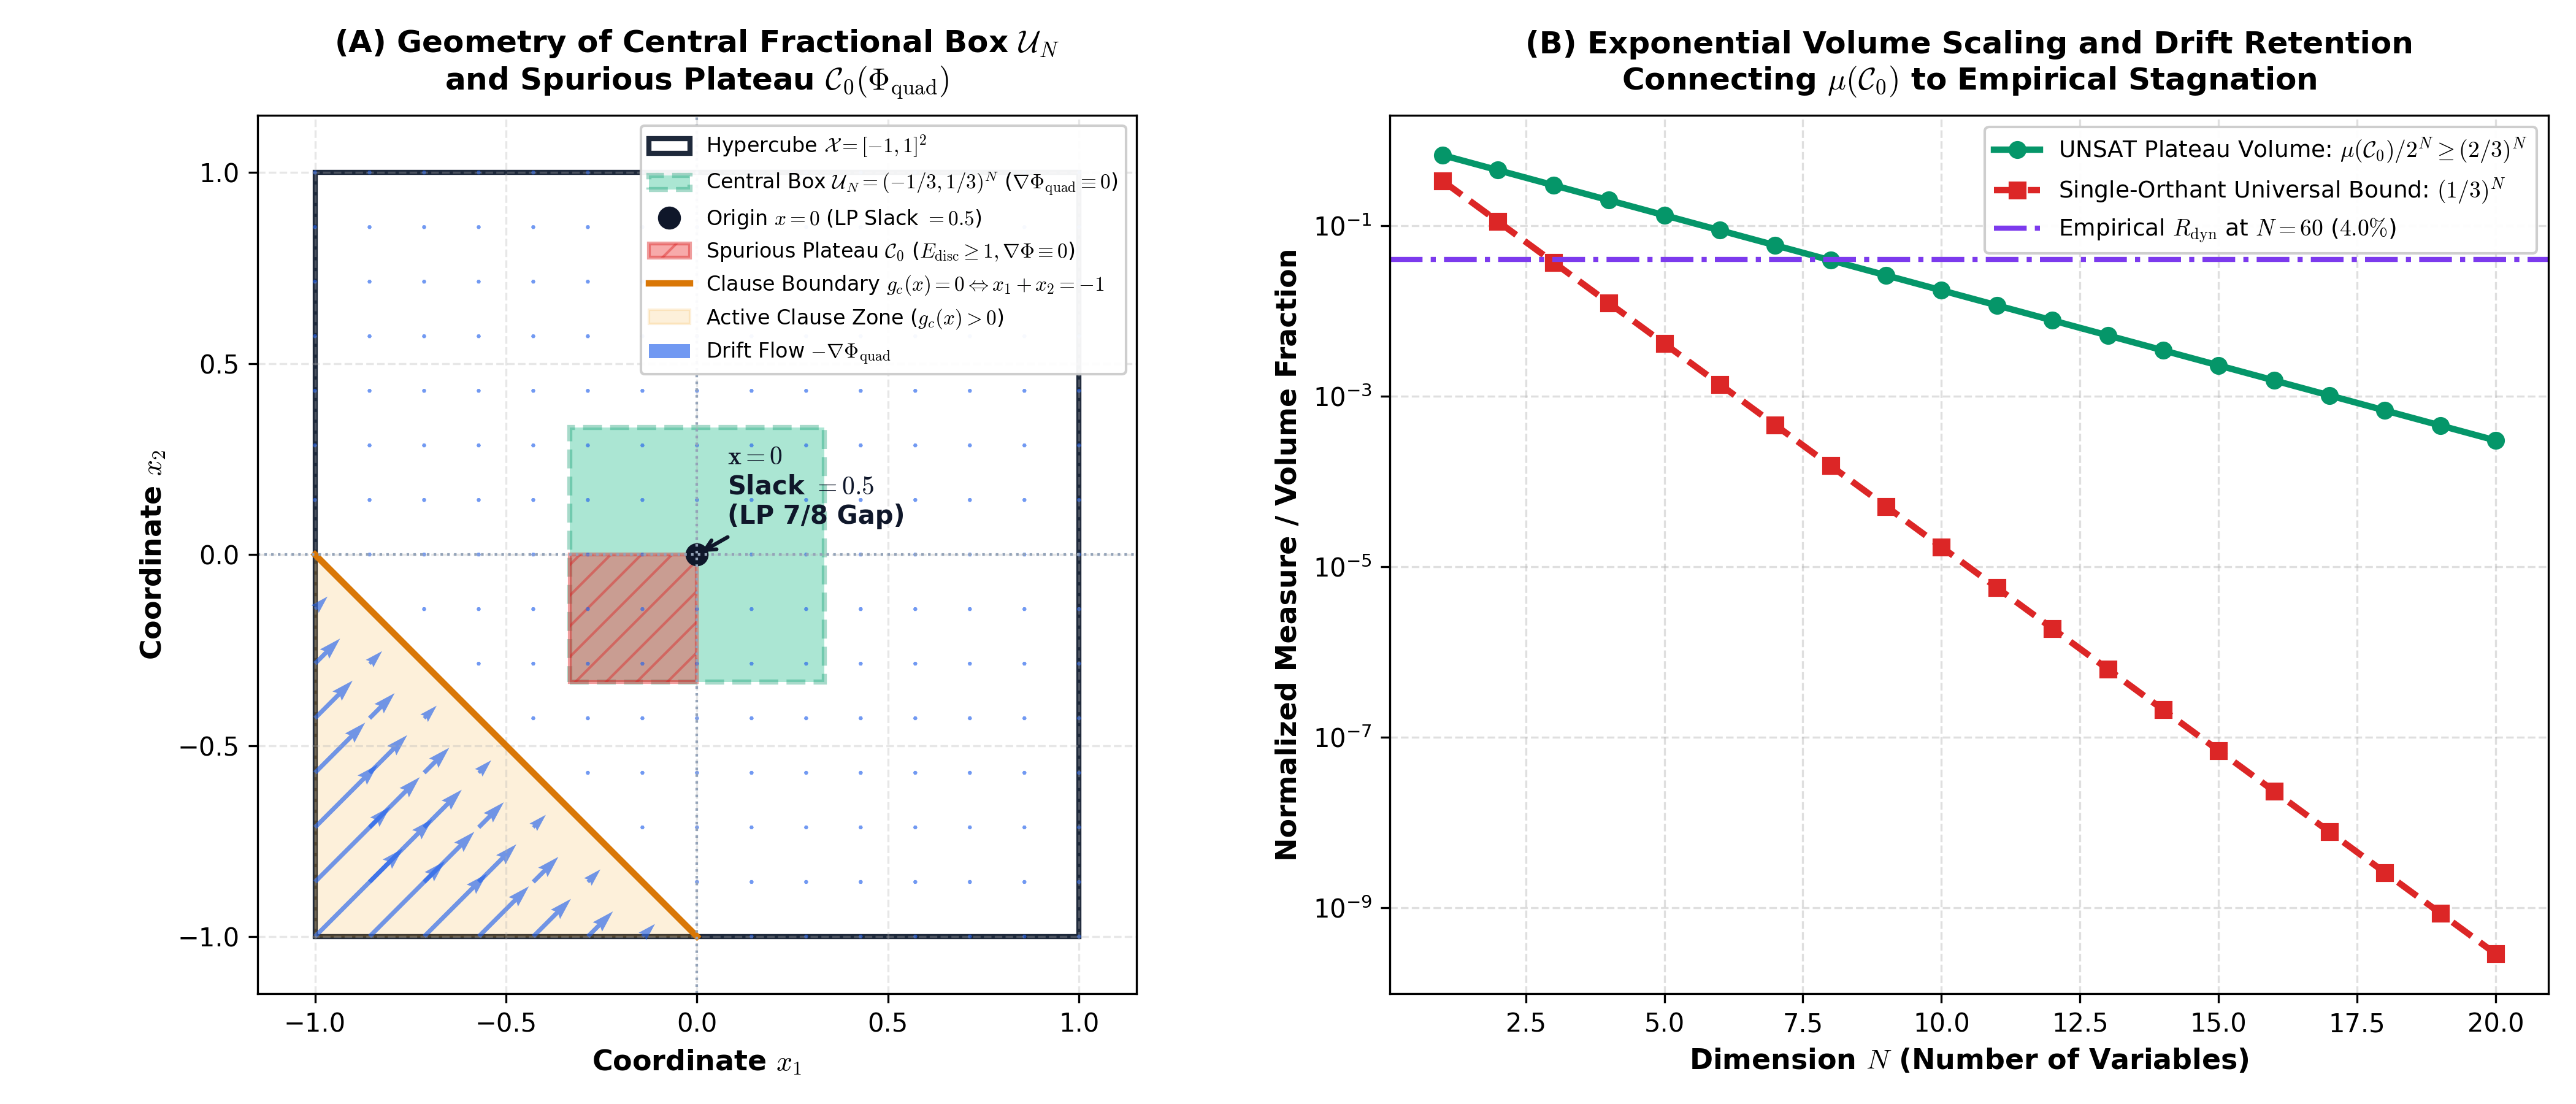
\includegraphics[width=0.80\textwidth]{../../fig_clg_teorema1_caixa_fracionaria.png}
\caption{Source figure from the audited CLG-R manuscript illustrating the central fractional box and its exponential-volume scaling. The theorem used here is the deterministic inclusion $\mathcal U_N\subseteq Z$.}
\end{figure}
\section{Measure-zero critical sets outside the Hinge plateau}
\begin{theorem}[Analytic critical sets]
If the Boolean energy is non-constant, then
\[
\mu\{\nabla\Phi_{\mathrm{mult}}=0\}=0,\qquad \mu\{\nabla\Phi_{\mathrm{soft}}=0\}=0.
\]
\end{theorem}
\begin{proof}
The multilinear potential is a non-constant polynomial. Hence at least one partial derivative is a nonzero polynomial, whose zero set has Lebesgue measure zero \cite{okamoto1973distinctness,caron2005zero}; the full critical set is contained in it.

The Softplus potential is real analytic. Its Hessian factorization below implies
\[
\Delta\Phi_{\mathrm{soft}}(x)=\frac34\sum_{c=1}^M w_c(x)>0,
\]
so it is non-constant. At least one partial derivative is therefore a nontrivial real-analytic function, and its zero set has measure zero \cite{krantz2002primer}.
\end{proof}
\section{Harmonicity of the multilinear extension}
\begin{theorem}[Harmonic saddle structure]
The multilinear potential satisfies $\Delta\Phi_{\mathrm{mult}}\equiv0$. Consequently it has no interior local minimum. Every non-degenerate interior critical point is a hyperbolic saddle with at least one positive and one negative Hessian eigenvalue, and every interior critical point has lower-energy points in every neighborhood.
\end{theorem}
\begin{proof}
Each clause term is multilinear in distinct variables, so every pure second derivative $\partial_{ii}^2\Phi_{\mathrm{mult}}$ vanishes. The Strong Minimum Principle excludes an interior local minimum for a non-constant harmonic function \cite{courant1962methods,evans2010partial}. At a non-degenerate critical point the symmetric Hessian is invertible with trace zero, forcing eigenvalues of both signs. The degenerate statement follows directly from the absence of a local minimum; a curve-selection argument may be used to strengthen this to a descending analytic arc \cite{milnor1968singular}.
\end{proof}
\begin{figure}[htbp]\centering
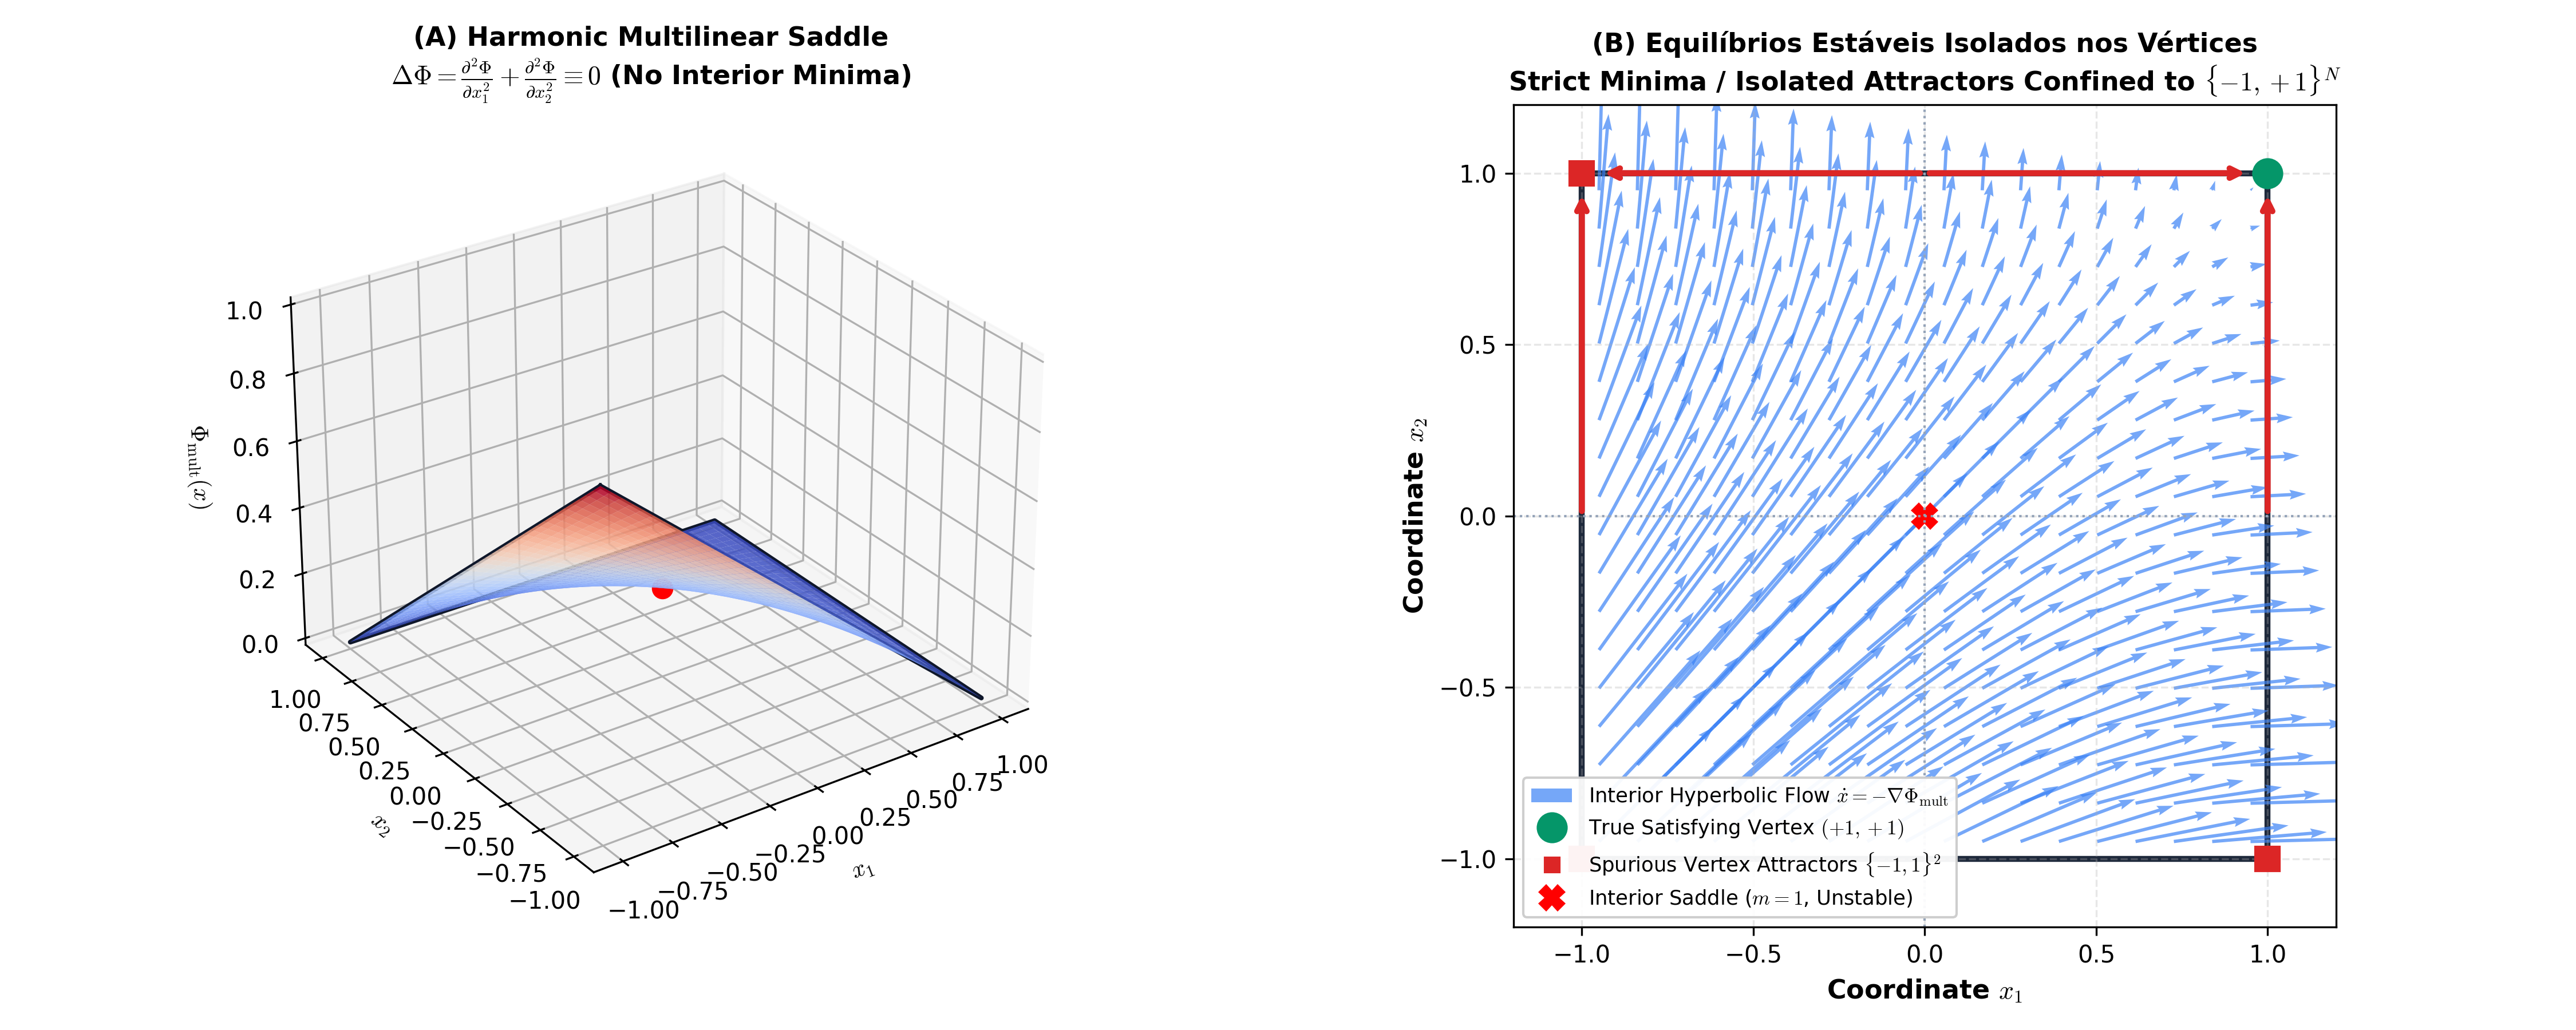
\includegraphics[width=0.80\textwidth]{../../fig_clg_teorema3_4_harmonic_saddles_vertices.png}
\caption{Source figure illustrating harmonic saddle geometry and confinement of isolated stable projected equilibria to Boolean vertices.}
\end{figure}
\section{Boundary faces and projected attractors}
The cube is stratified into relative interiors of faces. Fixing coordinates to $\pm1$ preserves multilinearity in the remaining coordinates, so the intrinsic Laplacian on each positive-dimensional face also vanishes.
\begin{theorem}[Face minima inherit vertex energy]
Let $x^*$ be a relative local minimum of $\Phi_{\mathrm{mult}}$ in the relative interior of a face $\mathcal F$. Then $\Phi_{\mathrm{mult}}$ is constant on $\mathcal F$, and
\[
\Phi_{\mathrm{mult}}(x^*)=E_{\mathrm{disc}}(v)\quad\text{for every Boolean vertex }v\in\mathcal V(\mathcal F).
\]
In particular, every strict local minimum relative to the full cube is a Boolean vertex.
\end{theorem}
\begin{corollary}[Isolated stable equilibria are vertices]
Under projected multilinear gradient flow, every isolated asymptotically stable equilibrium belongs to $\{-1,+1\}^N$.
\end{corollary}
\begin{proof}
Moreau projection gives
\[
\frac{d}{dt}\Phi_{\mathrm{mult}}(x(t))=-\|\Pi_{T_{\mathcal X}(x)}(-\nabla\Phi_{\mathrm{mult}})\|^2\le0.
\]
An isolated asymptotically stable equilibrium must be a strict local minimum: nearby lower-energy states cannot converge upward, while a distinct equal-energy point either decreases immediately below the equilibrium energy or is another equilibrium. The preceding theorem then forces a zero-dimensional face.
\end{proof}
The word isolated is essential. Positive-dimensional non-strict attracting continua may exist on boundary faces; the six-clause M6 construction provides an explicit example in a separate analysis.
\section{Softplus Hessian factorization and conditioning}
Let $V\in\mathbb R^{M\times N}$ have row $v_c^T=-\frac12(\sigma^{(c)})^T$. Define
\[
w_c(x)=\beta\sigma(\beta g_c(x))(1-\sigma(\beta g_c(x)))>0,\qquad W(x)=\operatorname{diag}(w_1,\ldots,w_M),
\]
where $\sigma(u)=(1+e^{-u})^{-1}$ is the logistic function.
\begin{theorem}[Exact Hessian factorization]
\[
\nabla^2\Phi_{\mathrm{soft}}(x)=V^TW(x)V\succeq0.
\]
Thus $\Phi_{\mathrm{soft}}$ is globally convex. If $\operatorname{rank}(V)=N$, it is strictly convex and
\[
\kappa(\nabla^2\Phi_{\mathrm{soft}})\le\kappa(W)\kappa(V^TV).
\]
\end{theorem}
\begin{proof}
Because $g_c(x)=v_c^Tx-1/2$,
\[
\nabla\Phi_{\mathrm{soft}}=V^T\sigma(\beta g),\qquad \nabla^2\Phi_{\mathrm{soft}}=V^TWV.
\]
For any $z$, $z^TV^TWVz=\|W^{1/2}Vz\|^2\ge0$. Courant--Fischer bounds then give the condition-number estimate when $V^TV$ is positive definite.
\end{proof}
\section{Softplus stiffness and finite precision}
Let $d_{\max}$ be the maximum number of clauses incident to a variable.
\begin{theorem}[Gradient Lipschitz scale]
Define $L_\beta=\sup_x\|\nabla^2\Phi_{\mathrm{soft}}(x)\|_2$. Then
\[
\frac3{16}\beta\le L_\beta\le\frac{3d_{\max}}{16}\beta.
\]
For $\mathcal U_N(\rho)=(-\rho,\rho)^N$ with $\rho<1/3$,
\[
\|\nabla\Phi_{\mathrm{soft}}\|_\infty\le\frac M2e^{-\beta(1-3\rho)/2},\qquad
\|\nabla\Phi_{\mathrm{soft}}\|_2\le\frac{\sqrt3M}{2}e^{-\beta(1-3\rho)/2}.
\]
\end{theorem}
\begin{proof}
Since $w_c\le\beta/4$,
\[
\|\nabla^2\Phi_{\mathrm{soft}}\|_2\le\frac\beta4\lambda_{\max}(V^TV).
\]
The absolute row sum of $V^TV$ for variable $i$ is at most $3d_i/4$, so Gershgorin gives the upper bound. If $g_c(x)=0$ for one clause, then $w_c=\beta/4$, and the rank-one summand has spectral value $(\beta/4)\|v_c\|^2=3\beta/16$, giving the lower bound. The central-box gradient estimates follow from $g_c\le-(1-3\rho)/2$ and $\sigma(u)\le e^u$ for $u\le0$.
\end{proof}
At the origin the relevant exponential scale is $e^{-\beta/2}$. The audited source distinguishes the ideal binary32 crossings of the minimum normal, minimum subnormal, and half-subnormal round-to-zero scales at approximately $174.67$, $206.56$, and $207.94$, and the corresponding binary64 values $1416.79$, $1488.88$, and $1490.27$. These are scales for the exponential factor, not implementation-independent thresholds for a particular sigmoid routine.
\begin{figure}[htbp]\centering
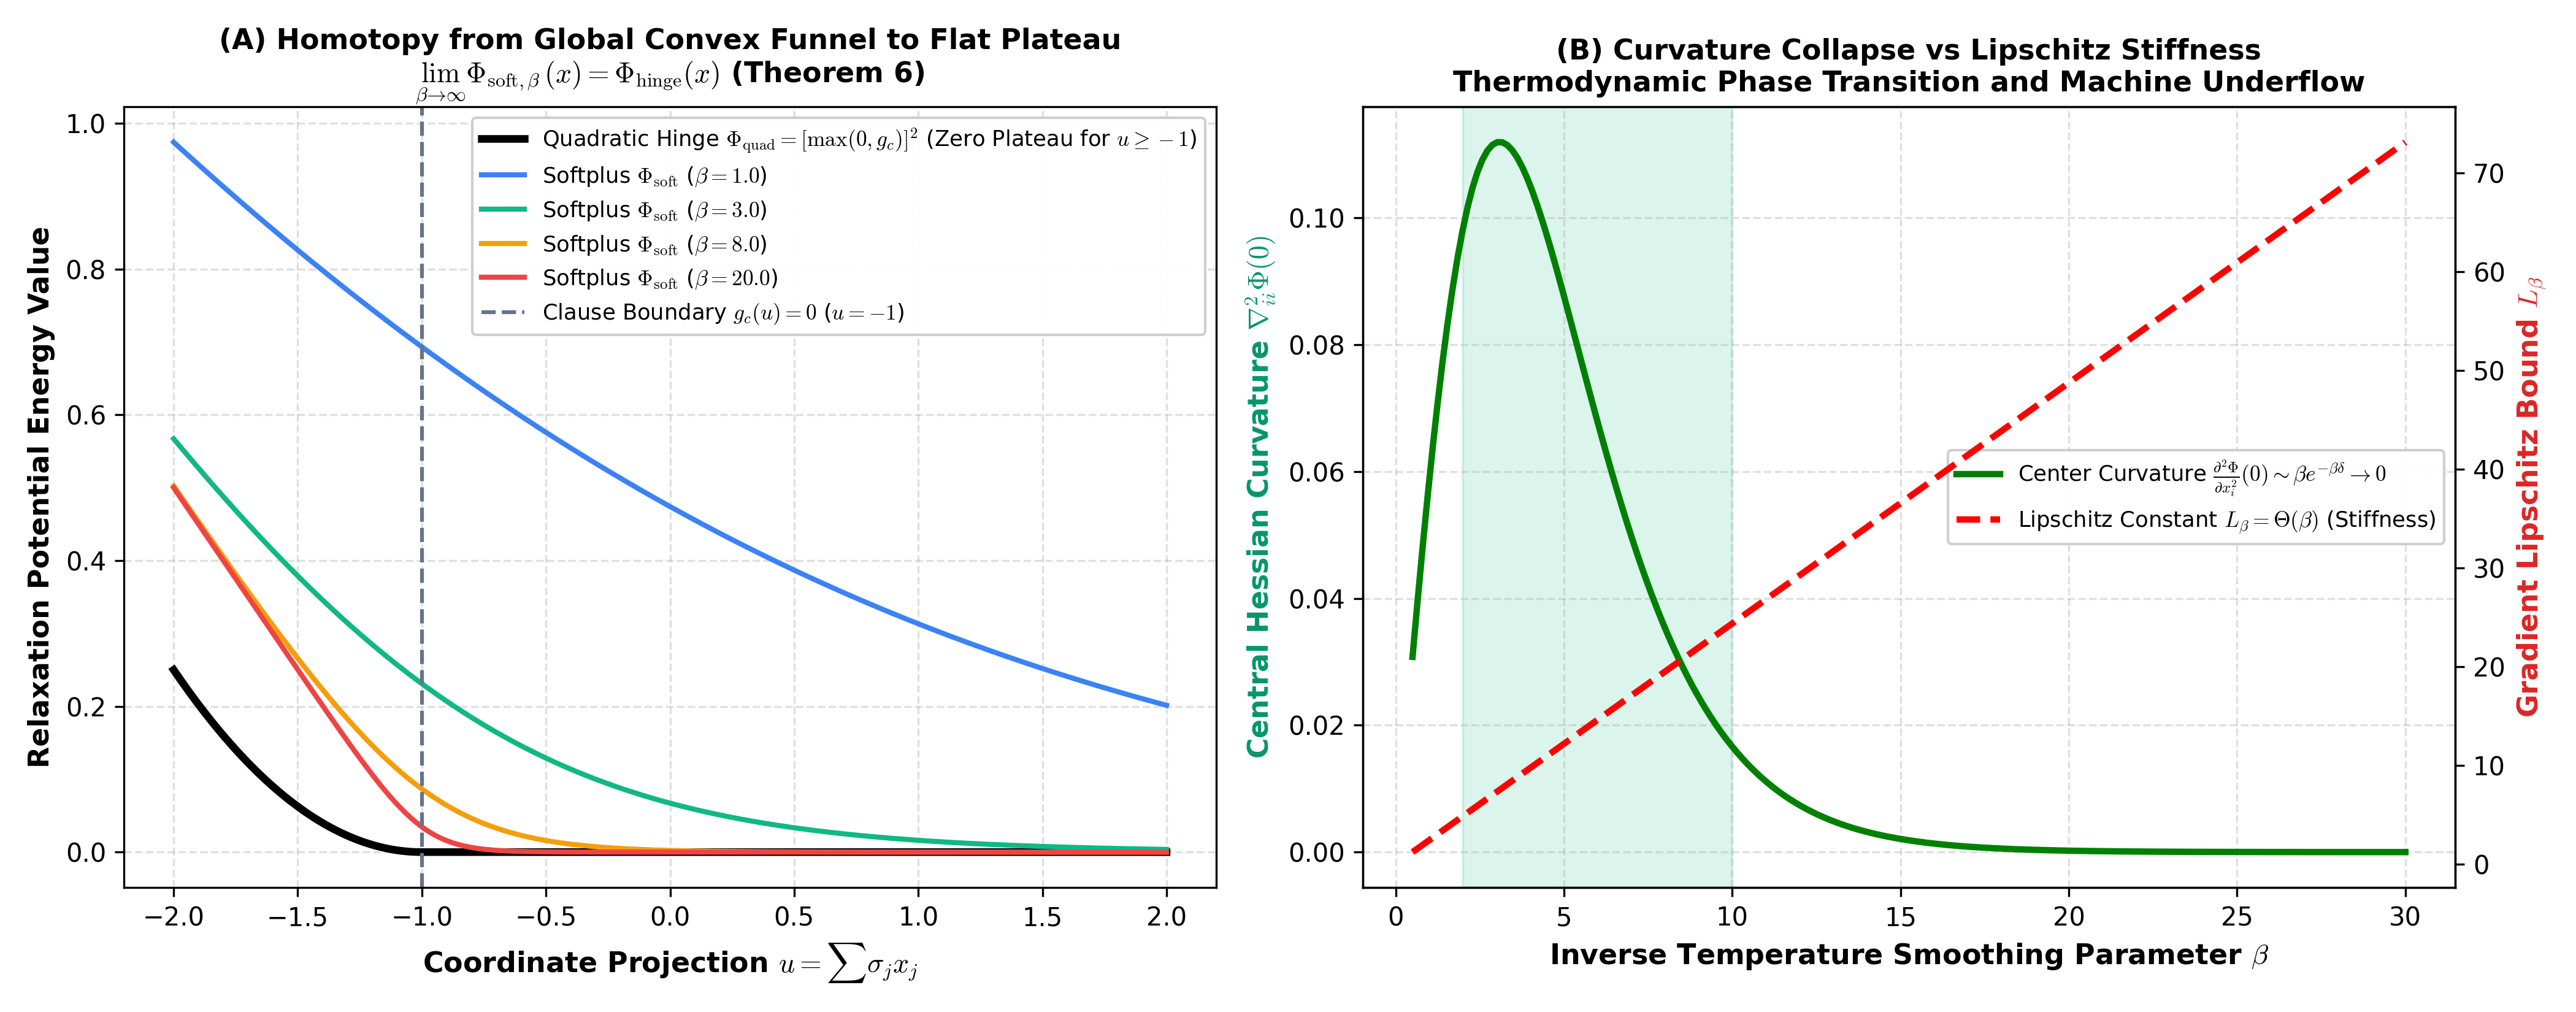
\includegraphics[width=0.80\textwidth]{../../fig_clg_teorema5_6_softplus_convexity_bifurcation.png}
\caption{Source figure illustrating the Softplus-to-Hinge homotopy and the coexistence of increasing global stiffness with vanishing central gradients as $\beta$ grows.}
\end{figure}
\section{Universal centripetal contraction of the squared Hinge flow}
Let
\[
Z=\{x\in\mathcal X:g_c(x)\le0\ \forall c\}
\]
be the clause-wise LP polytope.
\begin{theorem}[Centripetal contraction]
For every $x\notin Z$,
\[
\langle-\nabla\Phi_{\mathrm{quad}}(x),x\rangle=-\sum_{c\in\operatorname{act}(x)}(2g_c(x)^2+g_c(x))<0.
\]
Under projected flow the squared radius strictly decreases outside $Z$. Moreover the projected equilibrium set equals $Z$, and every trajectory satisfies $\operatorname{dist}(x(t),Z)\to0$.
\end{theorem}
\begin{proof}
For active $c$, $\sigma^{(c)}\cdot x=-(2g_c+1)$ and
\[
-\nabla\Phi_{\mathrm{quad}}=\sum_{c\in\operatorname{act}}g_c\sigma^{(c)},
\]
which yields the displayed inner product. Write $v=-\nabla\Phi=d+n$ by Moreau decomposition with $d=\Pi_Tv$ and $n\in N_X(x)$. For the box, $\langle x,n\rangle\ge0$, so $\langle x,d\rangle\le\langle x,v\rangle<0$. This excludes projected equilibria outside $Z$, while inside $Z$ all Hinge terms are inactive and the gradient vanishes. LaSalle's invariance principle for projected dynamical systems gives approach to $Z$ \cite{brogliato2006equivalence,nagurney1996projected}.
\end{proof}
\section{Synthesis}
The three representations implement sharply different interior geometries:
\begin{center}\small
\begin{tabularx}{\textwidth}{@{}lXXX@{}}
\toprule
& Hinge & Multilinear & Softplus\\\midrule
Central critical mass & positive plateau & measure zero & measure zero\\
Curvature & piecewise quadratic / flat & harmonic, zero trace & $V^TWV\succeq0$\\
Interior minima & plateau points & none & unique if $\operatorname{rank}(V)=N$\\
Projected equilibria & exactly LP polytope $Z$ & representation-dependent boundary set & minimizers of convex potential\\
Large-parameter issue & exact flatness & none of Softplus type & $L_\beta=\Theta(\beta)$ plus exponentially small central gradient\\
\bottomrule
\end{tabularx}
\end{center}
The comparison shows why Boolean agreement at the vertices is insufficient to predict continuous dynamics. The Hinge representation introduces a full-dimensional set of stationary fractional points; the multilinear representation removes interior minima but can still support non-strict boundary attractors; the Softplus representation restores convexity at the cost of a stiffness/vanishing-gradient tradeoff as $\beta$ increases.
\section{Conclusion}
Continuous 3-SAT relaxations that encode the same clauses can have fundamentally different critical geometry. The central fractional Hinge plateau, the harmonic multilinear extension, and the convex Softplus factorization provide three analytically distinct regimes. These deterministic results form a reusable geometric layer for later probabilistic or algorithmic investigations, but by themselves do not constitute a claim about computational complexity classes.
\begin{thebibliography}{9}
\bibitem{goemans1995improved} M. X. Goemans and D. P. Williamson, "Improved approximation algorithms for maximum cut and satisfiability problems using semidefinite programming," \emph{Journal of the ACM}, 42(6):1115--1145, 1995.
\bibitem{okamoto1973distinctness} M. Okamoto, "Distinctness of the eigenvalues of a quadratic form in a multivariate sample," \emph{Annals of Statistics}, 1(4):763--765, 1973.
\bibitem{caron2005zero} R. Caron and T. Traynor, "Zero sets of polynomials and Lebesgue measure," University of Windsor Technical Report, 2005.
\bibitem{krantz2002primer} S. G. Krantz and H. R. Parks, \emph{A Primer of Real Analytic Functions}. Birkh\"auser Boston, 2002.
\bibitem{courant1962methods} R. Courant and D. Hilbert, \emph{Methods of Mathematical Physics: Partial Differential Equations}, vol. 2. Interscience, 1962.
\bibitem{evans2010partial} L. C. Evans, \emph{Partial Differential Equations}, 2nd ed. American Mathematical Society, 2010.
\bibitem{milnor1968singular} J. Milnor, \emph{Singular Points of Complex Hypersurfaces}. Princeton University Press, 1968.
\bibitem{brogliato2006equivalence} B. Brogliato, A. Daniilidis, C. Lemar\'echal, and J. Malick, "Equivalence and complementarity issues in projected dynamical systems and differential inclusions," \emph{Mathematical Programming}, 107(3):317--335, 2006.
\bibitem{nagurney1996projected} A. Nagurney and D. Zhang, \emph{Projected Dynamical Systems and Variational Inequalities with Applications}. Springer, 1996.
\end{thebibliography}
\end{document}
